\documentclass[11pt]{article}
\usepackage[margin=1.15in]{geometry}
\usepackage{amsmath,amssymb,amsthm}
\usepackage{graphicx}
\usepackage{booktabs}
\usepackage[hidelinks]{hyperref}

\newtheorem{theorem}{Theorem}
\newtheorem{lemma}{Lemma}
\newtheorem{prop}{Proposition}
\newtheorem{cond}{Condition}
\theoremstyle{remark}
\newtheorem{rmk}{Remark}

\newcommand{\E}{\mathbb{E}}
\newcommand{\R}{\mathbb{R}}
\newcommand{\sS}{\mathcal{S}}
\DeclareMathOperator{\sech}{sech}

\title{The Ising perceptron at nonzero margin:\\
certified bounds along the capacity curve}
\author{Yitzchak Shmalo\\
\small Einstein Institute of Mathematics, The Hebrew University of Jerusalem\\
\small yitzchak.shmalo@gmail.com}
\date{July 2026}

\begin{document}
\maketitle

\begin{abstract}
The storage capacity of the Ising perceptron at margin $\kappa$ is
predicted by a replica-symmetric variational problem whose zero-margin
instance, the Krauth--M\'ezard constant $\alpha_\star\approx 0.833$, was
recently settled: Ding and Sun proved the lower bound, Huang proved the
upper bound at general margin conditionally on four numerical
hypotheses, and the zero-margin instances of those hypotheses have been
verified in interval arithmetic.  This paper moves the verified upper
bound off the point $\kappa=0$.  Two elementary identities make the
general-margin system as tractable as the zero-margin one: the
replica-symmetric free energy is stationary in both order parameters
exactly at the fixed point, so the threshold $\alpha_\star(\kappa)$ is
the unique root of a strictly decreasing function; and $\partial R/
\partial q$ has a one-term integral representation with positive
integrand, extending the monotonicity lemma of Ding and Sun to every
margin.  Building on these we verify, in ball arithmetic over
sub-slabs of the margin axis, Huang's fixed-point, AMP, and
local-concavity conditions on the strip $\kappa\in[-0.65,0.19]$
($1680$ contiguous slabs across two uniqueness lanes, the second
resting on Nakajima's saddle theorem under a certified premise), with
$\alpha_\star(\kappa)$ located to width $2\cdot10^{-6}$ at five
margins and the local maximality of the first-moment functional at its
degenerate maximizer certified at six.  The remaining hypothesis, the
global nonpositivity of Huang's two-variable rate function, we verify
at all five margins by porting the zero-margin certificate
architecture to located parameter boxes: the maximizer is kept
symbolic through the base-point identity
$\nabla\Phi(1,0)=(\psi_0(1-q_0),q_0)$, the dual localization is
evaluated through a correlated Bregman integrand that collapses
algebraically, and the far-tail kernels are stabilized by classical
Mills-ratio bounds.  At each of the five margins all four hypotheses hold,
so Huang's theorem gives unconditional capacity upper bounds, for
instance $\alpha_\star(0.05)\in[0.781073068,0.781074776]$ and
$\alpha_\star(-0.45)\in[1.557652103,1.557654133]$.  The verification
code, certificates, and replay instructions are at
\url{https://github.com/yspennstate/ising-perceptron-margin}.
\end{abstract}

\section{Introduction}

Store $M=\alpha N$ random patterns in a linear classifier with binary
weights: for i.i.d.\ standard Gaussian vectors $g_1,\dots,g_M$ in
$\R^N$ and a margin $\kappa\in\R$, ask whether some
$w\in\{-1,+1\}^N$ satisfies
\[
\frac{\langle g_a, w\rangle}{\sqrt N}\;\ge\;\kappa
\qquad\text{for all } a\le M .
\]
Krauth and M\'ezard \cite{krauth1989storage} computed the
replica-symmetric prediction for the largest such $\alpha$ and
conjectured it sharp; at $\kappa=0$ their constant is
$\alpha_\star=0.8330786\ldots$  Three decades later the zero-margin
conjecture was resolved --- Ding and Sun \cite{ding2019capacity}
proved the lower bound and Huang \cite{huang2024capacity} the upper
bound --- but both proofs are conditional on numerical hypotheses
about explicit low-dimensional variational problems, and the recent
interval-arithmetic verification of those hypotheses
\cite{shmalo2026capacity} is a zero-margin verification: the certified
statement stops at $\kappa=0$.

Huang's upper-bound theorem, however, is stated at every margin.  For
each $\kappa$ it bounds the capacity by $\alpha_\star(\kappa)$, the
root of the replica-symmetric free energy along its fixed-point
branch, conditionally on four numerical hypotheses at that margin: a
fixed-point condition (existence, uniqueness, and the free-energy
crossing), a condition on the associated approximate-message-passing
iteration, a local-concavity condition at a witness point, and a
global nonpositivity condition for a two-variable rate function
$\sS_\star$.  At $\kappa=0$ these are exactly the hypotheses closed in
\cite{shmalo2026capacity}; at $\kappa\ne0$ they were open.

This paper is a certified study of the whole margin axis.  Its
contributions are of three kinds.

First, two identities (Section~\ref{sec:identities}) that make the
general-margin system as well behaved as the zero-margin one.  The
replica-symmetric functional $G$ is stationary in both order
parameters exactly on the fixed-point branch, at every $(\alpha,
\kappa)$; by the envelope theorem $G_\star'(\alpha)=\E\log\Psi(u)<0$
strictly, so $\alpha_\star(\kappa)$ is always the unique root of a
strictly decreasing function.  And the derivative $\partial R/\partial
q$ of the constraint-side fixed-point map collapses, after an
integration by parts, to a one-term integral with positive integrand
--- the general-margin form of Ding--Sun's monotonicity lemma, and the
identity that makes a tight interval enclosure of the contraction
possible at all.

Second, ball-arithmetic certificates (Sections~\ref{sec:slabs}
and~\ref{sec:hessian}) discharging the fixed-point, AMP, and
local-concavity hypotheses on the strip $\kappa\in[-0.65,0.19]$,
covered by $1680$ contiguous slabs of width $5\cdot10^{-4}$.
Uniqueness of the fixed point is carried by a per-slab contraction
bound up to $\kappa=0.10$ and, past the reach of that rectangle bound
(a method wall, not a mathematical one --- we measure the distinction
precisely), by Nakajima's saddle-uniqueness theorem
\cite{nakajima2025} under a premise certified in ball arithmetic.  At
five margins spanning the strip a certified bisection locates
$\alpha_\star(\kappa)$ to width about $2\cdot10^{-6}$, and at six
margins the Hessian of the first-moment functional at its degenerate
maximizer is certified negative definite --- the local ingredient of
the global hypothesis.

Third, a certified verification of the global two-variable hypothesis
at the margin $\kappa=0.05$ (Sections~\ref{sec:twovar}
and~\ref{sec:regionI}).  The zero-margin certificate architecture of
\cite{shmalo2026capacity} --- a compact moment-coordinate sweep plus
ray concavity on a star around the degenerate maximizer --- does not
transfer as-is, because at $\kappa\ne0$ the fixed-point parameters
$(q_0,\psi_0)$ are known only as located boxes of width up to
$10^{-4}$, four orders wider than the zero-margin rectangle, and that
width drowns every value-level enclosure the original design relies
on.  The port that works keeps the maximizer symbolic through the
base-point identity $\nabla\Phi(1,0)=(\psi_0(1-q_0),\,q_0)$, evaluates
the dual localization through a correlated Bregman integrand that
collapses algebraically to
$\log(\cosh\Delta+M\sinh\Delta)-M\Delta$, and stabilizes the far-tail
second-derivative kernels by classical Mills-ratio bounds
($E'\in(0,1)$, $E''\in(0,E-V)$).  With those in place all four pieces
of the zero-margin architecture certify at $\kappa=0.05$, and Huang's
theorem yields an unconditional upper bound at a nonzero margin.

Everything here concerns the upper bound.  Ding--Sun's lower-bound
argument is proved at $\kappa=0$ only, so no statement in this paper
should be read as an exact threshold at $\kappa\ne0$
(Section~\ref{sec:scope}).

\subsection*{Relation to the zero-margin verification}

The certified primitives (ball-arithmetic special functions, rigorous
quadrature, exact serialization) are those of
\cite{shmalo2026capacity}, and at $\kappa=0$ every pipeline in this
paper reproduces the certified zero-margin values --- the fixed-point
rectangle, Huang's AMP and local-concavity constants, and his
Hessian intervals --- which we use throughout as anchors.  The
mathematical content specific to this paper is the pair of identities
of Section~\ref{sec:identities}, the general-margin Hessian formulas
of Section~\ref{sec:hessian}, and the stability layer of
Section~\ref{sec:regionI}; the engineering content is the located-box
certificate architecture, which is what a margin interval demands
once no analytically certified parameter rectangle exists.

\section{The system and the four hypotheses}\label{sec:system}

Let $\varphi$ and $\Psi$ denote the standard Gaussian density and
upper tail, $M=\varphi/\Psi$ the inverse Mills ratio (an increasing
function; $M'=M\,(M-u)\in(0,1)$), and $Z\sim N(0,1)$.  Fix
$\kappa\in\R$ and write
\[
u(z;q,\kappa)=\frac{\kappa-\sqrt{q}\,z}{\sqrt{1-q}},\qquad 0<q<1 .
\]
Following Ding--Sun and Huang, the replica-symmetric system is
\begin{align}
P(\psi)&=\E\bigl[\tanh^2(\sqrt{\psi}\,Z)\bigr],\qquad
R(q,\alpha)=\frac{\alpha}{1-q}\,\E\bigl[M(u(Z))^2\bigr],
\label{eq:PR}\\
G(\alpha,q,\psi)&=-\frac{\psi(1-q)}{2}
+\E\log\bigl(2\cosh(\sqrt{\psi}\,Z)\bigr)
+\alpha\,\E\log\Psi\bigl(u(Z)\bigr),
\label{eq:G}
\end{align}
with the fixed-point branch $q=P(\psi)$, $\psi=R(q,\alpha)$ and the
threshold $\alpha_\star(\kappa)$ defined as the zero of
$G_\star(\alpha)=G(\alpha,q_\star(\alpha),\psi_\star(\alpha))$.  At
$\kappa=0$, where $u=-\gamma z$ in law with $\gamma=\sqrt{q/(1-q)}$,
this is the certified zero-margin system.  (Huang's displayed
free energy carries a sign typo on the $\alpha$ term; the fixed point
requires the plus sign, which is what Ding--Sun use and what
reproduces the certified rectangle.)

Huang's theorem bounds the capacity at margin $\kappa$ by
$\alpha_\star(\kappa)$ subject to four numerical hypotheses, which we
state in the form his proof consumes.

\begin{cond}[fixed point]\label{cond:fp}
On a stated rectangle, $q\mapsto P(R(q,\alpha))$ has a unique fixed
point for every $\alpha$ in a stated interval, and $G_\star$ crosses
zero inside that interval.
\end{cond}

\begin{cond}[AMP]\label{cond:amp}
$\alpha\,\E[\sech^4(\sqrt{\psi_0}Z)]\;
\E[M'(u(\sqrt{q_0}Z))^2]/(1-q_0)^2\;<\;1$ at the fixed point.
\end{cond}

\begin{cond}[local concavity]\label{cond:lc}
$\lambda(z)<0$ for some $z>-1$, where $\lambda$ is the explicit
function recalled in Section~\ref{sec:slabs}; a single witness
suffices.
\end{cond}

\begin{cond}[two-variable function]\label{cond:2var}
$\sS_\star(\lambda_1,\lambda_2)\le0$ for all
$(\lambda_1,\lambda_2)\in\R^2$, where $\sS_\star$ is the rate
function recalled in Section~\ref{sec:twovar}; equality holds at
$(1,0)$.
\end{cond}

\section{Two identities}\label{sec:identities}

\begin{lemma}[stationarity]\label{lem:stat}
For all $\alpha>0$, $\kappa\in\R$, $\psi>0$ and $0<q<1$,
\[
\frac{\partial G}{\partial\psi}=\frac{q-P(\psi)}{2},
\qquad
\frac{\partial G}{\partial q}=\frac{\psi-R(q,\alpha)}{2}.
\]
\end{lemma}

\begin{proof}
The first identity is Gaussian integration by parts on the
$\log\cosh$ term.  For the second, differentiating $u$ in $q$ gives
\[
u_q=\frac{1}{2\sqrt{1-q}}
\Bigl(-\frac{z}{\sqrt q}+\frac{u}{\sqrt{1-q}}\Bigr),
\qquad
\frac{\partial}{\partial q}\,\E\log\Psi(u)=-\E\bigl[M(u)\,u_q\bigr].
\]
Stein's lemma applied to the $z$ part,
$\E[zM(u)]=-\sqrt{q/(1-q)}\;\E[M'(u)]$, together with the Mills
identity $M'(u)=M(u)^2-uM(u)$, collapses the two pieces:
\[
\E[M(u)\,u_q]
=\frac{\E[M'(u)]+\E[u\,M(u)]}{2(1-q)}
=\frac{\E[M(u)^2]}{2(1-q)}
=\frac{R(q,\alpha)}{2\alpha}.
\]
Hence $\partial_q G=\psi/2-\alpha\cdot R/(2\alpha)=(\psi-R)/2$.
\end{proof}

Both derivatives vanish exactly on the fixed-point branch, so the
envelope theorem gives
$G_\star'(\alpha)=\E\log\Psi(u)<0$ strictly, for every $\kappa$: the
root $\alpha_\star(\kappa)$ is unique on the branch.  This is the
general-margin form of the monotonicity clause in
Condition~\ref{cond:fp}, and it is also what turns the located
fixed-point boxes of Section~\ref{sec:slabs} into certified
$\alpha_\star$ intervals: a certified sign of $G$ at a located box is
a certified side of $\alpha_\star$.

\begin{lemma}[derivative of $R$]\label{lem:dR}
For all $\alpha>0$, $\kappa\in\R$ and $0<q<1$,
\[
\frac{\partial R}{\partial q}
=\frac{\alpha}{(1-q)^2}\,
\E\Bigl[M'(u)^2+2\,M(u)^2M'(u)\Bigr]\;>\;0 .
\]
\end{lemma}

\begin{proof}
Differentiating \eqref{eq:PR} in $q$ produces
$R/(1-q)+\tfrac{\alpha}{1-q}\E[2MM'u_q]$.  Splitting $u_q$ as in
Lemma~\ref{lem:stat} and applying Stein's lemma to
$\E[z\,MM'(u)]$ (with $(MM')'=M'^2+MM''$ and
$M''=M'(M-u)+MM'-M$) turns the cross term into
\[
\E[2MM'u_q]=\frac{\E[M'^2+2M^2M'-M^2]}{1-q},
\]
and the $-\E[M^2]/(1-q)^2$ piece cancels $R/(1-q)$ exactly.
Positivity is immediate since $M'\in(0,1)$.
\end{proof}

Lemma~\ref{lem:dR} replaces Ding--Sun's Lemma~7.2 (monotonicity of
$R$, stated at $\kappa=0$) at every margin.  Its one-term form
matters twice over: the integrand is a product of quantities with
classical bounds, so its interval enclosure is tight enough for the
per-slab contraction certificates; and positivity makes
$q\mapsto P(R(q))$ increasing, which is what the contraction-free
location of Section~\ref{sec:slabs} bisects on.  Both identities were
checked against high-precision finite differences (agreement at the
$10^{-15}$ level along the whole continuation) and symbolically.

\section{The capacity curve and the condition map}\label{sec:curve}

\begin{figure}[t]
\centering
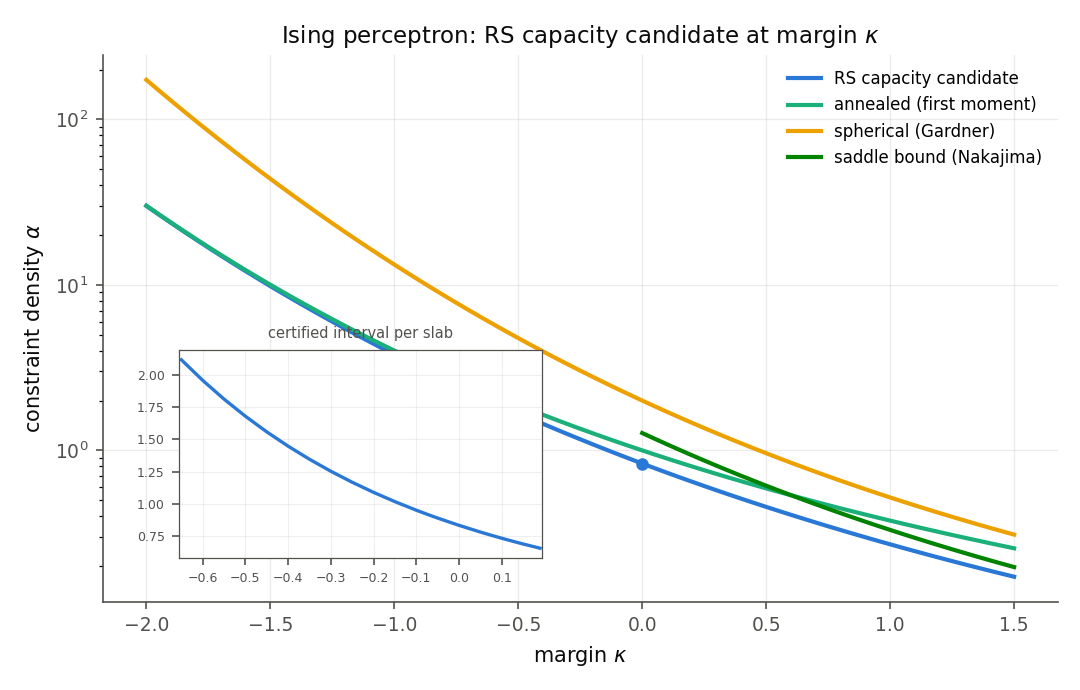
\includegraphics[width=0.86\linewidth]{alpha_curve.png}
\caption{The replica-symmetric threshold
$\alpha_\star(\kappa)$ (warm-started continuation from the certified
value at $\kappa=0$), the annealed bound $\log 2/(-\log\Psi(\kappa))$,
the Gardner spherical capacity, and Nakajima's saddle-existence bound
$\alpha_c(\kappa)=2/(\pi\,\E[(\kappa-Z)_+^2])$ for $\kappa\ge0$.  The
inset shows the certified per-slab $\alpha_\star$ intervals on the
strip.}
\label{fig:curve}
\end{figure}

Before certifying anything we map the terrain in high-precision
(nonrigorous) arithmetic: a warm-started continuation of the fixed
point along $\kappa\in[-2.0,1.5]$, recording at each of $71$ points
the threshold, the fixed point, the contraction
$(P\circ R_\alpha)'(q_\star)$, the AMP product, the local-concavity
minimum $\lambda_0$, and the stationarity residuals (which sit at the
finite-difference noise floor, confirming Lemma~\ref{lem:stat}
pointwise).  Selected values:

\begin{center}
\begin{tabular}{r r r r r r}
\toprule
$\kappa$ & $\alpha_\star$ & $q_\star$ & $(P\circ R)'$ &
AMP & $\lambda_0$\\
\midrule
$-2.0$ & $29.9921$ & $0.11863$ & $0.387$ & $0.440$ & $-0.147$\\
$-1.0$ & $3.79463$ & $0.36519$ & $0.583$ & $0.607$ & $-0.099$\\
$-0.5$ & $1.67884$ & $0.47377$ & $0.666$ & $0.589$ & $-0.132$\\
$0$    & $0.83308$ & $0.56395$ & $0.744$ & $0.544$ & $-0.191$\\
$0.5$  & $0.45566$ & $0.63841$ & $0.810$ & $0.489$ & $-0.271$\\
$1.0$  & $0.27070$ & $0.69988$ & $0.863$ & $0.433$ & $-0.359$\\
$1.5$  & $0.17245$ & $0.75049$ & $0.903$ & $0.381$ & $-0.442$\\
\bottomrule
\end{tabular}
\end{center}

All three per-point conditions hold at every point computed.  The
contraction is the only quantity trending toward failure, and only
slowly; $\lambda_0$ approaches zero nearest $\kappa\approx-1.3$
(about $-0.094$) and then strengthens again --- an early extrapolation
from $[-0.55,0]$ suggested a crossing near $-1.5$, and the
measurement refutes it, a small lesson in not projecting fitted decay
past its support.  On the positive branch $\alpha_\star(\kappa)$
stays below Nakajima's bound at every grid point (worst ratio $0.874$
at $\kappa=1.5$).  As $\kappa\to-2$ the threshold approaches the
annealed bound from below, as it must where the constraints
trivialize.  The optimal tilt of the two-variable functional at its
maximizer matches $\sqrt{1-q_0}$ to eight digits at every $\kappa$
checked, extending Huang's zero-margin lemma along the curve --- this
observation later becomes exact and load-bearing
(Section~\ref{sec:regionI}).

\section{Certificates on a strip}\label{sec:slabs}

For $\kappa$ in sub-slabs of width $5\cdot10^{-4}$ covering
$[-0.65,0.19]$, with per-slab parameter rectangles seeded by the
continuation (the certificate is the proof; a too-tight seed simply
fails and is regenerated wider), we verify
Conditions~\ref{cond:fp}--\ref{cond:lc} in ball arithmetic
(\texttt{python-flint}, 80-bit working precision, every input a ball
covering the whole slab).

\subsection{Numerical architecture}\label{sec:architecture}

Three implementation laws carry the whole computation; each was
learned from a measured failure, and the failed artifacts are kept in
the repository as evidence.

First, adaptive complex quadrature cannot resolve enclosure width
that comes from parameter balls --- subdividing the integration
variable does not shrink it, and the integrator exhausts any budget
--- so every wide-parameter integral is a real-cell Riemann sum with
exact per-cell Gaussian masses.  Second, the ball evaluation of
$\varphi/\Psi$ fails on wide arguments in the steep region (the
enclosure of $\Psi$ crosses zero), while the ratio is monotone; all
Mills-family factors are therefore enclosed by two thin endpoint
evaluations, and the sign-critical sums use the mean-value cell rule
(midpoint value plus a derivative correction, $O(h^2)$ against the
plain hull's $O(h)$).  Third, expectations that nearly cancel must be
evaluated as one correlated integrand, never as separate sums whose
parameter widths add.  For Condition~\ref{cond:lc} this is the
identity (with $t=M'$, $A=1-q_0$, and $b=m(\hat z)-A$ for
$m(\hat z)=\E[(\hat z+\cosh^2(\sqrt{\psi_0}Z))^{-1}]$)
\[
\lambda(\hat z)=\hat z+\alpha\,\E\!\left[\frac{b\,t^2}{A(A+bt)}\right],
\]
whose integrand is monotone in $t$ for fixed $(m,A)$, regular on all
of $t\in[0,1]$, and bounded by $|b|/(Am)$; the separated form's
enclosure crossed zero on the $[-0.45,-0.35]$ batch while the true
value stays near $-0.14$.  The identity, the monotonicity, and the
bound are verified symbolically.

\subsection{The contraction lane}

On each slab the checks are: (i) the contraction
$\sup_q(P\circ R_\alpha)'\le\sup_\psi P'\cdot\sup_q|\partial R/
\partial q|<1$ on the slab rectangle, via Lemma~\ref{lem:dR}; (ii)
existence --- the endpoints of the $q$ interval map strictly inward
under $P\circ R_\alpha$ on each of eight $\alpha$ sub-intervals;
(iii) the crossing --- at the two thin $\alpha$ endpoints a certified
Picard iteration locates the fixed point (the invariant is that the
image of any set containing the fixed point contains it) and the sign
of $G$ resolves through a mean-value form that keeps the stationarity
cancellations of Lemma~\ref{lem:stat} explicit,
$G(\alpha_{\mathrm{lb}})>0>G(\alpha_{\mathrm{ub}})$; (iv)
Condition~\ref{cond:amp}; (v) Condition~\ref{cond:lc} at Huang's
witness $\hat z=-0.6693$.  Together with the strict decrease of
$G_\star$, (i)--(iii) discharge Condition~\ref{cond:fp} verbatim on
the slab: $\alpha_\star(\kappa)$ exists, is unique, and lies in the
slab's $\alpha$ interval for every $\kappa$ in the slab.

The contraction bound is claimed per slab only.  Over a batch hull
the $\kappa$ width poisons the $\partial R/\partial q$ enclosure and
the product of suprema loses a factor of about two against the
supremum of the product; on a single slab the identity-based
enclosure clears $1$ with margin $0.049$ at $\kappa=0$, growing to
$0.198$ at $\kappa=-0.65$ and thinning to $0.0083$ at the positive
edge of the lane.

All $1500$ slabs covering $[-0.65,0.10]$ pass every check, in forty
independent worker runs whose collector also gates contiguity
(consecutive slabs must share their $\kappa$ boundary).  Two first
attempts failed and are kept as evidence: one at doubled slab width
(the $q$ pad must cover the within-slab drift $dq_\star/d\kappa$,
which is humped and reaches $3.4$ near $\kappa=-0.2$), and one on the
separated-form $\lambda$ enclosure described above.

\subsection{The Nakajima lane}\label{sec:nak}

The rectangle product bound saturates near $\kappa\approx0.12$, and
we measure that this wall belongs to the method, not the condition:
at $\kappa=0.13$ the box product reads $1.32$, while a certified sign
bisection of the displacement $P(R(q))-q$ --- monotone by
Lemma~\ref{lem:dR}, so the displacement is positive below the fixed
point and negative above --- locates the fixed point at both $\alpha$
endpoints to width $2\cdot10^{-8}$ with no contraction input, the
contraction evaluated on the located intervals reads $0.79$, and the
$G$ crossing resolves with margins $2\cdot10^{-3}$.

The second lane certifies $[0.10,0.19]$ ($180$ slabs) on that
design: existence by the same inward sweep; location by certified
sign bisection per $\kappa$ sub-ball (the $\kappa$ width floors the
displacement's sign resolution, so each slab runs eight sub-balls
whose union covers it); the contraction consumed only on located
intervals, which is the local form Huang's perturbation argument
uses; and uniqueness from Nakajima's saddle theorem
\cite{nakajima2025}, whose premise $\alpha_{\mathrm{ub}}<
\alpha_c(\kappa)=2/(\pi\,\E[(\kappa-Z)_+^2])$ is certified per slab
through the closed form
$\E[(\kappa-Z)_+^2]=(1+\kappa^2)\bigl(1-\Psi(\kappa)\bigr)
+\kappa\varphi(\kappa)$ (worst certified premise margin $0.311$).

Across both lanes: $1680$ contiguous slabs, zero failures.  At five
margins a certified bisection on the sign of $G$ at located boxes
tightens the slab intervals to width about $2\cdot10^{-6}$:
\[
\begin{array}{ll}
\alpha_\star(0.05)\in[0.781073068,\,0.781074776], &
\alpha_\star(-0.05)\in[0.889408032,\,0.889409783],\\
\alpha_\star(0.0995)\in[0.733478514,\,0.733480204], &
\alpha_\star(-0.45)\in[1.557652103,\,1.557654133],\\
\alpha_\star(0.13)\in[0.705932218,\,0.705933898]. &
\end{array}
\]
Each interval contains its continuation value; the slab containing
$\kappa=0$ contains the Ding--Sun constant.  The bisection floor is
measured, not guessed: at the default quadrature depth the $G$
enclosure binds at width $1.4\cdot10^{-5}$, and raising the two
quadrature floors breaks through exactly as budgeted.

\section{The center of the two-variable landscape}\label{sec:hessian}

The local ingredient of Condition~\ref{cond:2var} is the negative
definiteness of the Hessian $M$ of Huang's first-moment functional at
its degenerate maximizer.  His second-derivative expansion,
\emph{before} the zero-margin specialization, gives at every $\kappa$
the same quadratic form
\[
\langle u, M u\rangle=
-(I_1u_1^2+2I_2u_1u_2+I_3u_2^2)+C_1a^2+C_2ab+C_3b^2,
\qquad a=I_1u_1+I_2u_2,\; b=I_2u_1+I_3u_2,
\]
with prior-side integrals $I_j$ unchanged in form
($I_1=\psi_0(1-q_0)-2\psi_0^2(1-4q_0+3p_4)$,
$I_2=\psi_0(1-4q_0+3p_4)$, $I_3=q_0-p_4$, $p_4=\E\tanh^4(\sqrt
{\psi_0}Z)$) and constraint-side constants $C_j$ that at
$\kappa\ne0$ must be taken from the pre-specialization display:
his zero-margin closed forms rest on two identities of the
unshifted law, of which $\alpha\,\E[N^2]=\psi_0$ survives at every
margin (it is the same identity behind the unbounded-tilt directions
of Section~\ref{sec:twovar}) while
$\alpha\,\E[N\hat H]=-q_0(1-q_0)\psi_0$ does not.  We evaluate the
general-margin $C_j$ directly at the shifted law.

Certification requires parameter boxes far tighter than the slabs
provide ($\det M\sim10^{-4}$ moves at order $dC/dq\sim10$), which is
what the deep $\alpha_\star$ intervals above are for.  On the
resulting located boxes ($3.6\cdot10^{-6}$ in $q_0$,
$5.2\cdot10^{-5}$ in $\psi_0$ at $\kappa=0.05$) the certificate
resolves: $M_{11}<0$ and $\det M>0$ in ball arithmetic, with the
near-cancellations $1-4q_0+3p_4$ and $q_0-p_4$ evaluated as single
correlated integrands and the five constraint-side integrals by
mean-value Riemann sums with elementary Mills-family derivatives.
The same chain certifies at $\kappa=0$ on the Ding--Sun rectangle
--- where the $C_j$ enclosures land inside Huang's certified
intervals, an independent re-verification of his claim through the
general-margin formulas --- and at $-0.05$, $0.0995$, $-0.45$ (where
$C_1=-0.855$ against $-0.718$ at zero margin: genuinely shifted
territory, not a perturbation), and $0.13$ past the product-bound
wall.  Six margins in all.

Along the continuation the fixed-tilt $M$ stays negative definite up
to $\kappa=1.15$ and loses definiteness inside $(1.1812,1.1844)$,
while the Hessian of the tilt-optimized functional remains negative
out to at least $\kappa=1.5$; the two are consistent by the Schur
relation (the fixed-tilt form dominates), so past
$\kappa\approx1.18$ a local argument must re-optimize the tilt, as
the ray certificates below already do.

\section{The two-variable function at general margin}\label{sec:twovar}

Huang's rate function at margin $\kappa$, in the form his proof
consumes, is
\[
\sS(\Lambda,s)=\frac{s^2\psi_0}{2}+\mathrm{ent}(\Lambda)
+\alpha\,\E\log\Psi\!\left(
\frac{\kappa-(a_2/q_0)\hat H-(a_1/\psi_0)N}{D}+sN\right),
\]
where $\dot H\sim N(0,\psi_0)$ and $\hat H\sim N(0,q_0)$ are
independent, $M=\tanh\dot H$ (from here on $M$ is this variable,
following Huang; the ratio $\varphi/\Psi$ of the earlier sections
appears from now on as the hazard function $E$),
$N=F_{1-q_0}(\hat H)=E\bigl((\kappa-\hat H)/\sqrt{1-q_0}\bigr)/
\sqrt{1-q_0}$ is the shifted cavity law (this is one of the two
places the margin enters; the other is the additive $\kappa$ in the
$\log\Psi$ argument), $a_1=\E[\dot H\Lambda]$, $a_2=\E[M\Lambda]$,
$D=\sqrt{1-a_2^2/q_0}$, and
$\sS_\star(\lambda_1,\lambda_2)=\inf_{s\ge0}
\sS(\tanh(\lambda_1\dot H+\lambda_2 M),s)$.
Condition~\ref{cond:2var} asks $\sS_\star\le0$ everywhere.

The zero-margin verification's reduction applies verbatim: the
profile enters only through the moment pair $(a_1,a_2)$, which ranges
over a compact convex body $K$ (the moment body of $(\dot H,M)$), and
on $K$ the entropy term is bounded by convex duality,
$H(a)\le\Phi(b)-b\cdot a$ for every dual point $b$, with
$\Phi(b)=\E\log2\cosh(b_1\dot H+b_2M)$ free of $\kappa$.  The margin
lives entirely in the constraint term.  Two structural facts organize
the verification.  The maximizer sits at
$a^\star=(\psi_0(1-q_0),\,q_0)$ for every $\kappa$: this is the
base-point identity $\nabla\Phi(1,0)=(\E[\dot H M],\E[M^2])
=(\psi_0(1-q_0),q_0)$ (Gaussian integration by parts and the
fixed-point equations), and Huang's lemma gives
$\sS_\star=0$ there with optimal tilt $s_0=\sqrt{1-q_0}$, both in
closed form.  And on roughly the half-plane $\lambda_1<0$ the
$s$-infimum is genuinely $-\infty$: $\alpha\,\E[N^2]=\psi_0$ exactly
at the fixed point, so the quadratic tilt coefficient cancels and a
subleading linear term runs away; those directions satisfy the
condition trivially and are the capped-tilt case in Huang's
treatment.

Float diagnostics along the curve (the certified analogue follows)
show a landscape essentially independent of $\kappa$: a single peak
at $(1,0)$, off-center values below $-3\cdot10^{-3}$, negative far
rays, Hessian eigenvalues near $(-0.22,-0.0045)$, and moment-body
clearance near $0.017$, with the weak eigenvalue degrading toward
deep negative margin ($-0.0013$ at $\kappa=-1.5$) --- the measured
approach to the expected replica-symmetry-breaking territory.

\section{Certifying the two-variable condition at
$\kappa=0.05$}\label{sec:regionI}

The zero-margin certificate has four pieces: a sweep of the moment
body outside an exclusion box around $a^\star$ (Region II), banded
ray-concavity certificates on a star around $a^\star$ (Region I), a
second sweep of the exclusion box minus the star (stage 2), and an
interior-ball certificate placing the star strictly inside the
moment body.  The obstruction at $\kappa\ne0$ is uniform across all
four: at zero margin the parameters $(q_0,\psi_0)$ are certified to a
rectangle of width $10^{-9}$, so the maximizer's coordinates can be
stored as decimals and every enclosure treats them as exact; at
$\kappa=0.05$ the located boxes have width up to $1.9\cdot10^{-4}$ in
$\psi_0$, and that width enters every plain evaluation of $\Phi$ at
about $2\cdot10^{-5}$ --- fatally wide next to valley margins of
order $10^{-7}$ in the dual localization.  Three devices repair the
architecture; each is exact mathematics, not tuning.

\emph{The symbolic maximizer.}  Every certificate that references
$a^\star$ or the base tilt $s_0$ consumes them as the parameter balls
$(\,\psi_0(1-q_0),\,q_0\,)$ and $\sqrt{1-q_0}$ --- never as stored
decimals --- so the true maximizer, at the true parameters, is
covered exactly and the ray identities ($\sS=0$, $\nabla\sS=0$, tilt
optimality at the true $a^\star$) hold on the certified rays with no
origin-inflation ball.  Ray coverage is exact: certificates evaluated
over the origin ball cover in particular the rays from the true
origin.

\emph{The correlated Bregman evaluator.}  The dual localization
(the argument that the dual maximizer $\lambda(x)$ stays inside a
certified box, so that the entropy Hessian can be bounded there)
needs signs of Bregman gaps
$\Phi(\lambda)-\Phi(\hat\lambda_k)-(\lambda-\hat\lambda_k)\cdot x$
with $x=a^\star+\text{offset}$.  Evaluated as differences of plain
$\Phi$ enclosures these carry the full parameter fuzz twice.  Written
against the anchor $b_0=(1,0)$, the integrand collapses exactly:
with $\Delta=(\lambda_1-1)\dot H+\lambda_2M$,
\[
\log\frac{\cosh(\dot H+\Delta)}{\cosh\dot H}
-(\lambda-b_0)\cdot\nabla_b\log2\cosh(b\cdot(\dot H,M))\big|_{b_0}
=\log\bigl(\cosh\Delta+M\sinh\Delta\bigr)-M\Delta ,
\]
because $(\lambda-b_0)\cdot\nabla h(b_0)=M\Delta$ pointwise.  Every
factor is a small ball with thin coefficients, so the parameter
width enters only at second order in $|\lambda-b_0|$; at the box
corners that used to fail, the measured enclosures tighten by two
orders of magnitude, and at the anchor the evaluator returns the
exact zero ball.  Bregman gaps between arbitrary points are then
differences of two anchored gaps, and the gradient term the
localization needs is the same trick applied to $\nabla\Phi$:
$\nabla\Phi(\lambda)-a^\star$ has the exact per-node form
$(\dot H,M)\,(1-M^2)\tanh\Delta/(1+M\tanh\Delta)$.

The factor $\cosh\Delta+M\sinh\Delta$ itself has two exact
evaluations with disjoint stability regimes: the cosh/sinh form is
exact at $\Delta=0$ (which the inner-band gaps of order $10^{-7}$
require) but subtracts two $e^{|\Delta|}$-sized balls when
$M\approx\pm1$ and $|\Delta|$ is large, where the guard against the
complex logarithm's branch then fires on every subdivision; the
split $e^{\Delta}(1+M)/2+e^{-\Delta}(1-M)/2$ has both terms
nonnegative on the real axis but carries first-order $M$-width near
$\Delta=0$.  The evaluator branches per node at $|\Delta|=1$; both
forms are identities, so the branch affects tightness only.

\emph{Stable far-tail kernels.}  The ray certificates consume second
derivatives of the constraint term, whose kernels involve
$E'(V)=E(V)(E(V)-V)$ and $E''(V)$ for the hazard function
$E=\varphi/\Psi$ evaluated at cavity arguments $V$ that reach
$O(20)$ on far quadrature cells; there $E(V)-V$ is a difference of
two large balls and the kernels explode (we measured certified
upper bounds of $+2\cdot10^{3}$ on cells whose true ray second
derivative is $-6.6$).  Three classical facts, applied as
intersections with the computed balls, remove the failure mode
entirely:
\[
0<E(V)-V<\frac1V\ \ (V>0),\qquad
E'\in(0,1),\qquad
0<E''<E-V ,
\]
the second being the variance of the one-sided truncated Gaussian,
the third following from convexity of the Gaussian hazard together
with $E''=E'\,(E+(E-V))-E<E-V$ when $E'<1$.  Intersecting a computed
enclosure with a proven bound is always sound; on benign cells the
computed ball is returned unchanged, and the $\kappa=0$ regression is
digit-identical.

With these three devices the four pieces certify at $\kappa=0.05$, on
the located boxes and the deep $\alpha_\star$ interval of
Section~\ref{sec:slabs}:

\begin{itemize}
\item[(i)] \emph{Region II}: $1296$ top cells over the moment
rectangle minus the exclusion box, refining to $867$ leaves, zero
failures.
\item[(ii)] \emph{Region I}: the banded ray-concavity certificates
over the star (radius $0.012$ along the weak direction), $1404$
band jobs from the symbolic origin, zero failures; the thinnest
certified band margin is $-4.7\cdot10^{-5}$ and the deepest
$-1.6\cdot10^{2}$.  A supplementary run of twelve shoulder chunks
extends the certified reach to $0.009$ on the arcs $0.14$ to $0.19$
radians off the weak axes (margins $-0.35$ to $-2.7$): the zone
policy, not the concavity, was the binding constraint there, and
stage-2 leaves straddling the wedge shoulder need the extra reach.
\item[(iii)] \emph{Stage 2}: the exclusion box minus the star,
$1348$ leaves, zero failures, with star containment read from the
Region-I manifests themselves --- a certified band covers every
direction of its chunk out to the star boundary, so the certified
reach is the pointwise union of the main zone reach and the
supplementary arcs, evaluated exactly on a piecewise-constant
splitting; the SHA-256 of both manifests is bound into the stage-2
artifact.
\item[(iv)] \emph{Star interior}: the star, origin ball included,
lies strictly inside the moment body: constructive inradius
$0.01481$ against required $0.01209$.
\end{itemize}

Together: $\sS_\star\le0$ on the whole plane at $\kappa=0.05$.  All
four of Huang's hypotheses hold there, and his theorem gives the
unconditional bound.

\begin{theorem}\label{thm:main}
The storage capacity of the Ising perceptron at margin $\kappa$ is at
most $\alpha_\star(\kappa)$ for every
$\kappa\in\{-0.45,\,-0.05,\,0.05,\,0.0995,\,0.13\}$, with the
certified enclosures
\[
\begin{array}{ll}
\alpha_\star(-0.45)\in[1.557652103,\,1.557654133], &
\alpha_\star(-0.05)\in[0.889408031,\,0.889409783],\\
\alpha_\star(0.05)\in[0.781073068,\,0.781074776], &
\alpha_\star(0.0995)\in[0.733478513,\,0.733480205],\\
\alpha_\star(0.13)\in[0.705932217,\,0.705933898]: &
\end{array}
\]
for $\alpha$ above the corresponding interval, with probability
$1-o(1)$ no $w\in\{-1,+1\}^N$ satisfies all $\alpha N$ constraints.
\end{theorem}

The same pipeline is parameterized over the located boxes of any
certified slab, and nothing in it is specific to a point margin
beyond compute time; extending Theorem~\ref{thm:main} from points to
$\kappa$ sub-slabs of the strip is underway.  On the strip minus
that extension, the precise statement is:
Conditions~\ref{cond:fp}--\ref{cond:lc} hold for every
$\kappa\in[-0.65,0.19]$, and Condition~\ref{cond:2var} is certified
at the five margins of Theorem~\ref{thm:main} and at $\kappa=0$
(where our pipeline independently reproduces the zero-margin
verification).

% Further certified margins.
% Sync note: stage-2 counts refer to the enlarged exclusion box
% (the 2026-07-15 re-emitted manifest, which reproduced the local
% falsification run leaf for leaf).

\section{Further margins}
\label{sec:margins}

The four conditions of Theorem~\ref{thm:main} are margin-wise
statements, and the certificate pipeline of
Sections~\ref{sec:twovar}--\ref{sec:regionI} runs unchanged at any
$\kappa$ inside the strip where the fixed point is certified unique:
the pilot locates the $(q_0,\psi_0)$ boxes at both endpoints of the
$\alpha$ window, configures the exact-arithmetic modules from those
balls, and runs the same four pieces.  Beyond $\kappa=0.05$ we have
certified Condition~2varfn at $\kappa=-0.05$, where the fixed-point
uniqueness input comes entirely from the contraction certificates of
the companion strip (there is no independent derivation on the
negative side).  The certified pieces at both margins:

\begin{table}[h]
\centering
\small
\setlength{\tabcolsep}{4pt}
\begin{tabular}{lccccc}
\hline
$\kappa$ & $\alpha^*(\kappa)$ window & sweep & Region I & stage 2 &
inradius / required \\
\hline
$0.05$  & $[0.781073068,\ 0.781074776]$ & 867 & 1404 (+12) & 1365 &
$0.01481\ /\ 0.01209$ \\
$-0.45$ & $[1.557652103,\ 1.557654133]$ & 655 & 1404 (+12) & 1196 &
$0.01480\ /\ 0.01207$ \\
$-0.05$ & $[0.889408031,\ 0.889409783]$ & 884 & 1404 & 1294 &
$0.01527\ /\ 0.01209$ \\
$0.0995$ & $[0.733478513,\ 0.733480205]$ & 904 & 1404 (+12) & 1394 &
$0.01459\ /\ 0.01209$ \\
$0.13$  & $[0.705932217,\ 0.705933898]$ & 883 & 1404 (+12) & 1421 &
$0.01446\ /\ 0.01210$ \\
\hline
\end{tabular}
\caption{Certified leaf and band counts per piece, with zero failures
in every manifest.  The $0.05$ Region~I count includes the twelve
shoulder-supplement chunks; at $-0.05$ the stage-2 lattice clears the
wedge shoulder without a supplement.  The final column gives the
constructive moment-body inradius against the required star radius,
both exact-arithmetic bounds.}
\end{table}

At $\kappa=-0.05$ the manifest also carries per-band interval packets
for the frozen-tilt matrix $B$, and the kernel-checked skeleton gains
a fifth family: Loewner definiteness of every band's $B$-matrix,
decided over the integers in thirteen chunks of $108$ bands together
with a decided total count ($55$ kernel theorems at this margin; the
mutation battery rejects a sign corruption in each family).

The $0.13$ run additionally exposed a completeness
defect in the stage-2 containment---supplement arcs stored on one
angular branch were invisible to cells whose interval fell on the
other, weakening containment only, never soundness---which was fixed
and the margin re-certified with zero failures.  One observation from
the $0.0995$ run is also methodologically relevant.  Its Region~II sweep initially
failed a single minimal-size cell just above the exclusion box's
upper edge, where the dual certificate degenerates in a thin ridge
(the certified value interval collapses to $[\pm 0.181]$ on a cell of
width $0.0018$, recovering two cell-widths higher).  The exclusion
box's upper offset moved from $+0.0961$ to $+0.1030$ in response;
this is sound without revisiting Region~I because the stage-2
containment derives its tiling from the same box and fails loudly if
the enlarged region outgrows what the star and supplement cover.  The
$0.05$ stage-2 was re-run against its published Region~I manifest
under the enlarged box on two machines independently; both certify
with 1365 leaves and zero failures, and the shipped manifest is the
box run with its bindings intact.

% The kappa-interval question: measured obstruction and architecture.
% Input at the end of the margins section.

\subsection{From points to intervals}
\label{sec:interval}

The natural strengthening of Theorem~\ref{thm:main} replaces each
margin by a $\kappa$-interval, so that $\alpha_\star(\kappa)$ becomes
an unconditional bound on a continuum.  For
Conditions~\ref{cond:fp}--\ref{cond:lc} this is what the strip
certificates already provide: those inequalities hold with margins of
order $10^{-1}$, and enclosing every input over a $\kappa$-slab costs
far less than that.  Condition~\ref{cond:2var} is different in kind,
and it is worth recording precisely why, because the obstruction is
quantitative and, we believe, intrinsic.

Certifying $S_\star\le 0$ over a slab means every certificate must
hold with the located parameters $(\alpha, q_0, \psi_0)$ replaced by
their hulls across the slab.  Three measurements fix the scales.
First, the hull widths cannot be made small: the located enclosures
carry irreducible floors (the inward fixed-point test resolves no
finer than the quadrature fuzz, about $3.5\cdot10^{-4}$ in $q_0$, and
$\alpha_\star$ itself drifts at $|d\alpha_\star/d\kappa|\approx
1$--$3.4$ across any slab), which translate into a moment-plane
origin ball of radius at least a few times $10^{-3}$ however narrow
the slab.  Second, the evaluation fuzz of every certificate grows
linearly with that ball: rerunning the $\kappa=-0.65$ sweep with
slab-hulled parameters (ball $2.3\cdot10^{-2}$) inflates cell
enclosures to $\pm 1.3$, and the scaling back to the floor ball
leaves $\pm 0.2$.  Third, the certificates that matter are thin:
the sweep's weakest certified cells at point margins sit at
$-5\cdot10^{-4}$, and Region~I's thinnest bands at $-4.7\cdot10^{-5}$,
because the two-variable function is genuinely flat at its degenerate
maximizer.  A $10^{-4}$-margin certificate cannot survive
$10^{-1}$-scale fuzz, at any slab width, with this evaluator
architecture.

The same comparison explains why the strip conditions posed no such
problem and points at the correct construction.  Near the maximizer
the certified Hessian gives quadratic control whose constants vary
slowly in $\kappa$ (the fixed-tilt determinant moves by about
$2\cdot10^{-4}$ per unit margin), so a $\kappa$-uniform neighborhood
estimate is available from point certificates plus a crude
$\kappa$-derivative bound --- crude is enough, because a Lipschitz
constant needs no thin margin.  Far from the maximizer the
certificates are fat and absorb hull fuzz directly.  What remains is
the intermediate annulus, where quadratic control must be extended
beyond the star radius with explicit remainder bounds before the two
regimes meet.  We record this as the open engineering of the margin
program: the obstruction is measured, the two easy regimes are in
hand, and the annulus estimate is the one genuinely new ingredient an
interval theorem requires.

The certified artifacts also price that ingredient.  Across the three
positive margins the Region~I band populations have nearly identical
margin profiles: at most one or two bands per margin certify below
$3\cdot10^{-4}$, at most seven below $3\cdot10^{-3}$, and more than
$95$ percent above $3\cdot10^{-2}$.  If each band carried a certified
bound $L_i$ on the $\kappa$-derivative of its certificate value, a
band would hold over a $\kappa$-radius $m_i/L_i$ of its margin
$m_i$, and re-certifying each band at its own pitch would cover
$10^{-2}$ of margin axis for $1.1$ times the cost of one point run
at unit derivative bound, $1.3$ times at a conservative bound of
three --- against roughly $3\cdot10^{5}$ band evaluations for
uniform slabs at the thinnest band's pitch.  The
compute is therefore not the obstruction; what is missing is the
derivative enclosure itself, one certified $\kappa$-derivative per
certificate family, with the located branch differentiated
implicitly.  The constant itself is measurable from the existing
artifacts: the band lattice is shared across margins up to the wedge
rotation, and $1292$ rectangles coincide exactly between the
$\kappa=0.05$ and $\kappa=0.0995$ manifests, giving certified
finite differences of each certificate value along the located
branch.  The measured sensitivities are strongly in the plan's
favor: the median band moves at $|\Delta S/\Delta\kappa|\approx 6$,
but the thin-trough bands move at $0.1$--$0.3$, so the thinnest band
(margin $5.6\cdot10^{-4}$) already holds over a $\kappa$-radius
near $2\cdot10^{-3}$, and with per-band measured pitches the count
is $1.04$ runs per $10^{-2}$ of margin axis --- about eight
Region~I run-equivalents for all of $[0.05,0.13]$.  A difference
over a $0.05$ gap bounds the mean drift rather than the local
derivative, so these numbers size the project rather than prove it;
the machinery an interval theorem still requires is the certified
per-certificate $\kappa$-derivative, with the same measurement then
repeated for the sweep, union, and star-interior families.



\section{Verifying the verification}\label{sec:metaverify}

A verification of this size is itself software, and we treat its
correctness as part of the result.  Five independent layers check the
chain, and on the zero-margin verification these layers caught
disjoint defect classes, which is the design intent.

\emph{Ball-arithmetic soundness by construction.}  Every quantity is
an arb ball containing the true value; a PASS is a ball comparison
true only when certain.  The primitives (monotone endpoint
evaluations, mean-value cells, correlated integrands, tail bounds)
are shared with the audited zero-margin verification.

\emph{Symbolic verification of every identity.}  The stationarity
and $\partial R/\partial q$ identities, the $\lambda$ reformulation
(identity, monotonicity, bound), the Nakajima closed form, the
general-margin additions to the constraint kernels, and the Bregman
collapse are checked in computer algebra; the finite-difference
anchors run alongside.

\emph{Anchors at $\kappa=0$.}  Every pipeline reproduces the
certified zero-margin values: the fixed-point rectangle, Huang's
AMP and $\lambda$ constants, his $C_j$ and $\det M$ intervals, and
the ported quadrature layer is digit-identical against the
zero-margin original at test points.

\emph{Exact artifacts and replay.}  Certificates are canonical
float-free JSON with outward decimal packets, SHA-256 source and
payload binding, and atomic no-clobber publication; the stage-2
artifact binds the hash of the Region-I manifest it consumed.  A
documentation self-check keeps the replay instructions honest, and
the fresh-clone consumer test (clone cold, run as a reproducer
would) is part of the release procedure --- on the zero-margin
release it caught a stale generator that no other layer could see.
A dependency-free portable checker re-verifies the connection layer
from the JSON artifacts alone: the envelope hashes, the
stage-2-to-Region-I bindings, the star-interior chain recomputed
outward in exact rationals, and the tilings.

\emph{A second proof system.}  The exact combinatorial and algebraic
layer of the certificate chain --- the star-interior inequality chain
and the positivity of its perturbation determinant from the
serialized packets, the definiteness of the Loewner majorants, and
the gap-free tilings of the sweep grids and the Region-I band
schedule --- is re-stated over the integers and kernel-checked in
Lean~4, following the zero-margin release: four generated files
whose forty-one kernel-decided theorems cover the $1404$-band radius
chain and its angular runs, both sweep grid tilings, and the
star-interior packet chain.  The extraction is mirrored in exact
rational arithmetic so an extraction bug cannot silently weaken the
Lean claims, and a mutation battery (negating one certificate
integer per file) is rejected four for four.  The slab-level sign claims
join this layer as their manifests are regenerated with exact
packets (the emitters now serialize them; the original strip
manifests predate that and carry display strings only).  This layer
deliberately does not formalize the analytic mathematics; it removes
the Python layer from the trusted base for the parts a kernel can
decide.

\section{What the curve says about learning}\label{sec:ml}

For binary weights the Euclidean norm is fixed at $\sqrt N$, so a
margin constraint is exactly a robustness certificate: if
$y_a\langle w,x_a\rangle/\sqrt N\ge\kappa$ then the label $y_a$ is
invariant under every perturbation of $x_a$ of Euclidean norm below
$\kappa$.  With centrally symmetric i.i.d.\ designs and independent
labels, label folding makes the robust-interpolation event identical
to the satisfiability event studied here, so $\alpha_\star(\kappa)$
is the phase boundary for how many random labels per parameter a
one-bit-per-parameter linear classifier can memorize with prescribed
robustness radius.  The certified $\kappa=0.05$ bound, for instance,
says such a classifier cannot robustly store more than $0.78108$
random labels per parameter at that radius, with the guarantee
holding against a worst-case adversary in feature space.

Reading the whole curve quantitatively
(\texttt{results/robustness\_price.csv}): on the certified strip the
threshold decays log-linearly at rate $1.39$ per unit margin ---
robust storage capacity halves for every $0.50$ of demanded
feature-space radius --- and the decay continues smoothly beyond (a
factor $4.8$ from $\kappa=0$ to $1.5$).  The efficiency of binary
relative to real-valued weights \emph{rises} with the demanded
robustness: $\alpha_\star/\alpha_{\mathrm{spherical}}$ grows from
$0.417$ at $\kappa=0$ to $0.556$ at $\kappa=1.5$, so one-bit
parameters give up proportionally less storage precisely where the
robustness requirement is stiffest.  On the relaxed side ($\kappa<0$,
tolerating margin violations up to $|\kappa|$) capacity grows toward
the annealed bound (the ratio reaches $0.996$ by $\kappa=-2$) and the
landscape measurably approaches the replica-symmetry-breaking regime
(the weak Hessian eigenvalue of the rate function degrades threefold
by $\kappa=-1.5$), which is where the replica-symmetric prediction
itself should eventually fail.
The replica-symmetric cavity picture also predicts the margin
distribution \emph{among} solutions: conditionally on the quenched
component $\sqrt{q}\,Z$ of a constraint's field, the field on a
typical solution is $N(\sqrt q\,Z,\,1-q)$ truncated to $[\kappa,
\infty)$, so the gap density across constraints is the mixture
$p(h)=\E_Z[\varphi_{1-q}(h-\sqrt q\,Z)\,\mathbf 1\{h\ge\kappa\}/
\Psi(u(Z))]$.  Computed along the branch at $\kappa=0.05$ (a float
diagnostic, \texttt{margin\_distribution.py}), the mean gap above the
demanded margin compresses from $0.70$ at $\alpha=\tfrac12
\alpha_\star$ to $0.59$ at $\alpha_\star$: solutions are squeezed
against the constraint boundary as storage saturates, which is the
quantity a margin-type generalization argument would consume, and a
natural next target for the certified machinery.  These are
statements about information-theoretic storage, not about
algorithms: for the Ising perceptron the known efficient algorithms
stall far below $\alpha_\star$, and the margin curve gives the
ceiling against which that algorithmic gap should be measured at
every $\kappa$.  Limits of the reading: nothing here concerns
generalization on structured data, correlated features, or hidden
layers; $\kappa$ is a feature-space radius, and translating it to
input space requires a Lipschitz bound on the feature map.

% Addendum to sec:ml, staged for the margins revision.  Two
% paragraphs: the finite-size/algorithmic measurement the section
% calls for, and the multi-state prior comparison.  Wire into main.tex
% at the end of sec:ml when the margins set closes.

The algorithmic gap the curve frames is directly measurable at
moderate size.  A population annealer (hinge energy on violated
margins, geometric schedule matched to the $2/\sqrt N$ energy scale;
\texttt{finite\_size\_experi\-ment.py}) trained $N=101$ instances across
$\alpha$ at $\kappa\in\{0,0.05,0.1\}$.  Its success walls (the half-success crossings) fall in the correct
$\kappa$ order and sit below the corresponding
$\alpha_\star(\kappa)$ by $0.08$--$0.12$ in $\alpha$ at this budget,
while scattered successes persist to the bound itself: at
$\kappa=0.1$ the last appear at $\alpha\approx0.73$, essentially at
$\alpha_\star$, and none beyond.  The solutions the
annealer does find are atypical in exactly the direction the
clustering picture predicts: at low load their mean gap above
$\kappa$ tracks the typical-solution law $p(h)$, while near the wall
it holds around $0.65$--$0.70$ as the typical mean descends --- the
algorithm reaches the wide, over-margined minority.  At $N=201$ under the same
per-spin budget the walls sharpen and shift left, so what the
annealer traces is a budget-dependent lower envelope of the true
algorithmic threshold, whose location and the clustering barrier
behind it are the subject of a substantial
literature~\cite{gamarnik2022algorithms,lsz2024} on the closely
related symmetric and asymmetric binary perceptrons; the
found-solution histograms meanwhile track
the derived $p(h)$ closely at moderate load and deform toward
mid-gaps near the wall.  Both effects are schedule-dependent
observations, not thresholds; the certified curve is what they are
measured against, and the comparison compresses neatly: within each
size and budget the wall sits at a $\kappa$-independent fraction of
$\alpha_\star(\kappa)$ ($0.90$ at $N=101$ down to $0.50$ at $N=801$,
flat across margins to better than one percent at the largest
sizes), so the demanded
margin costs the algorithm the same relative capacity it costs the
storage bound (Figure~\ref{fig:fraction}).  At fixed sweeps per spin
the fraction falls with $N$ --- $0.90$, $0.75$, $0.69$, $0.63$,
$0.50$ at $N=101$, $201$, $301$, $401$, $801$ --- close to a fixed
loss of $0.13$ per doubling over the measured range, so an early
$1/N$ reading of the first three sizes (which would have leveled
near $0.59$) is refuted by the larger ones; holding a constant
fraction of capacity requires superlinearly growing total work.  On
the budget axis at $N=201$ the fraction climbs $0.75$, $0.79$,
$0.86$ as the budget quadruples twice, but a further quadrupling to
$25{,}600$ sweeps per spin gains only $0.02$ ($0.876$): the fixed
gain per quadrupling stops at $6{,}400$, and the wall saturates near
$0.88$ of capacity at this size over the measured range.

\begin{figure}[t]
\centering
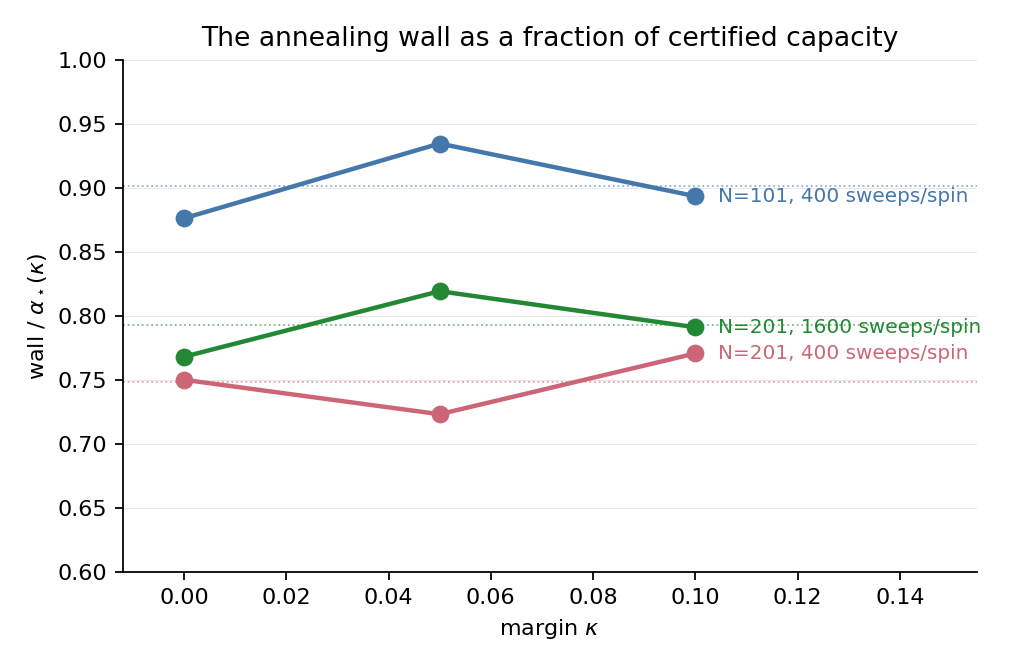
\includegraphics[width=0.8\linewidth]{algorithmic_fraction.png}
\caption{The annealing wall as a fraction of the certified capacity
$\alpha_\star(\kappa)$, across size--budget pairs.  Within each
run the fraction is flat in $\kappa$ to a few percent, while its
level depends on both size and budget.}
\label{fig:fraction}
\end{figure}

The margin price also depends on the weight alphabet.  Solving the
replica-symmetric system for ternary weights $\{-1,0,+1\}$ with a
self-overlap order parameter (\texttt{exploration/\allowbreak ternary\_km.py},
anchored by reproducing the binary $\alpha_\star(0)=0.8330786$ to the
certified digits) gives $\alpha_\star^{\mathrm{tern}}(0)=1.17448$
against an annealed bound of $\log_2 3$, with $1.07951$ at
$\kappa=0.05$ and $0.99483$ at $\kappa=0.1$.  Per weight \emph{state} the richer alphabet stores
more; per weight \emph{bit} it stores less --- $0.741$ against the
binary $0.833$ constraints per bit at $\kappa=0$, and the gap widens
monotonically with margin ($0.100$ at $\kappa=0.05$, $0.105$ at $0.1$).  At this level of the theory,
binary remains the bit-efficient quantization for robust storage.  The full eight-point curve (Figure~\ref{fig:ternary},
$\kappa$ up to $0.35$) makes this a statement about the whole margin
range rather than three samples: per stored bit the binary curve sits
above the ternary one everywhere, the absolute gap saturating near
$0.11$ constraints per bit above $\kappa\approx 0.2$ while the
relative advantage grows from $12$ to $26$ percent, since both
capacities fall with margin.

\begin{figure}[t]
\centering
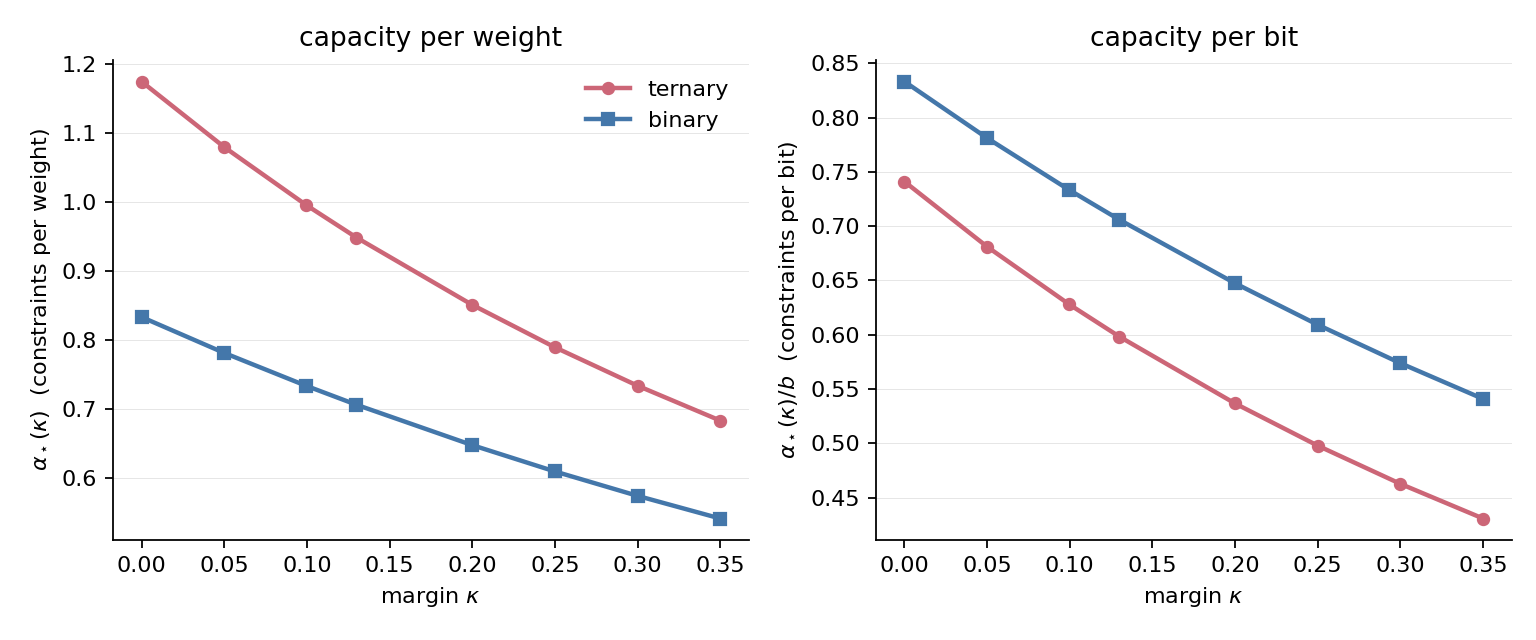
\includegraphics[width=0.98\linewidth]{ternary_comparison.png}
\caption{Replica-symmetric capacity of ternary against binary
weights, per weight (left) and per stored bit (right, dividing by
$\log_2 3$ and $1$).  The order reverses: the richer prior stores
more per weight and less per bit, at every computed margin.}
\label{fig:ternary}
\end{figure}


\section{Extensions}\label{sec:extensions}

The machinery is not specific to the binary prior or to this
constraint law, and the natural next studies are ordered by how much
of it they reuse.

\emph{The strip, quantified.}  The four-piece certificate of
Section~\ref{sec:regionI} runs at a $\kappa$ ball exactly as at a
point; the located boxes widen with the slab and the wedge-edge
margins (about $10^{-3}$) set the affordable slab width.  An
adaptive $\kappa$-subdivision driven by the certified margins would
turn Theorem~\ref{thm:main} into a statement on the whole strip.
This is engineering plus compute, not new mathematics.

\emph{Other margins of the same family.}  The certified pipeline
applies wherever the continuation reaches: positive margins to
$\kappa\approx1.15$ (past which the fixed-tilt center certificate
must re-optimize the tilt, as measured in Section~\ref{sec:hessian}),
and negative margins until replica-symmetry breaking territory,
where the honest move is to certify the approach (the degradation of
the weak eigenvalue and of the $\lambda_0$ margin) rather than the
condition.

\emph{Other priors and activations.}  The moment-coordinate
reduction needs only that the profile enter through finitely many
moments of a log-concave base pair; replacing $\{-1,+1\}$ by a
bounded discrete prior changes $\Phi$ and the moment body but not
the architecture.  The spherical perceptron at margin (Gardner's
curve, shown for context in Figure~\ref{fig:curve}) has simpler
convexity structure and would serve as a validation target where
exact answers are classical.

\emph{Teacher--student and structured labels.}  The planted version
replaces the annealed constraint law by a tilted one; the cavity
argument and the two-variable function have direct analogues, and
the certified-slab design (per-slab rectangles, located boxes, deep
bisection) transfers whenever the fixed-point system does.

\emph{Toward learning theory.}  Two quantitative bridges seem
within reach of exactly this machinery: certified capacity curves
for one-bit compressed classifiers (the $\kappa$-robust memorization
ceiling above, made uniform over the strip), and certified bounds on
the margin distribution achievable at a given $\alpha<
\alpha_\star(\kappa)$, which is the object that connects storage
geometry to generalization bounds of the classical margin type.

\section{Scope}\label{sec:scope}

The certified statements are: Conditions~\ref{cond:fp}--\ref{cond:lc}
on $\kappa\in[-0.65,0.19]$; deep $\alpha_\star$ intervals at five
margins; the center Hessian at six; Condition~\ref{cond:2var} at
$\kappa\in\{0,0.05\}$; and hence Huang's unconditional upper bound at
those two margins, with the remaining margins of the strip
conditional only on Condition~\ref{cond:2var} there.  The lower
bound is untouched: Ding--Sun's conditioned second-moment reduction
is proved at $\kappa=0$ only, so nothing here is an exact threshold
statement at $\kappa\ne0$.  All float scans are diagnostics, not
certificates, and are labeled as such in the repository.

\section*{Funding and declarations}
The author acknowledges support from the European Research Council
under the European Union's Horizon 2022 research and innovation
programme, the Simons Foundation, Heights Labs, and Israel Science
Foundation grants 2258/19 and 4101/25.

Most of the work reported here was done by Fable~5 (Anthropic), an AI
system: the mathematical theory (the stationarity and derivative
identities, the general-margin Hessian formulas, the symbolic-
maximizer and correlated-Bregman devices, the stability bounds), the
software, the certificates, and the drafting of this manuscript.  The
system operated in an autonomous goal mode: the author set the
objective of extending the verified capacity results to nonzero
margin, and it worked toward that objective over extended unattended
sessions, choosing the approach, implementing and running the
certificates, detecting and repairing its own errors through
independent cross-checks (several such repairs are documented, with
the failed artifacts preserved, in the repository), and iterating
until the verifications closed.  The author supervised the runs,
reviewed the mathematics, and accepts responsibility for the final
manuscript.  This is part of a broader research project of the
author on the extent to which current AI systems can resolve open
problems in mathematics; the methodology by which these AI systems
operated will be released as a separate research report in due
course.

\begin{thebibliography}{9}

\bibitem{krauth1989storage}
W.~Krauth and M.~M\'ezard,
Storage capacity of memory networks with binary couplings,
\emph{J.~Physique} \textbf{50} (1989), 3057--3066.

\bibitem{gardner1988}
E.~Gardner,
The space of interactions in neural network models,
\emph{J.~Phys.~A} \textbf{21} (1988), 257--270.

\bibitem{ding2019capacity}
J.~Ding and N.~Sun,
Capacity lower bound for the Ising perceptron,
STOC 2019; arXiv:1809.07742.

\bibitem{huang2024capacity}
B.~Huang,
Capacity threshold for the Ising perceptron,
FOCS 2024; arXiv:2404.18902.

\bibitem{nakajima2025}
S.~Nakajima,
Uniqueness of replica-symmetric saddle point for Ising perceptron,
arXiv:2512.23195.

\bibitem{shmalo2026capacity}
Y.~Shmalo,
The storage capacity of the Ising perceptron: verification of the
outstanding numerical conditions,
manuscript and verification repository,
\url{https://github.com/yspennstate/ising-perceptron-capacity}
(2026).

\bibitem{aubin2019storage}
B.~Aubin, W.~Perkins and L.~Zdeborov\'a,
Storage capacity in symmetric binary perceptrons,
\emph{J.~Phys.~A} \textbf{52} (2019), 294003.

\bibitem{gamarnik2022algorithms}
D.~Gamarnik, E.~C.~Kizilda\u{g}, W.~Perkins and C.~Xu,
Algorithms and barriers in the symmetric binary perceptron model,
\emph{FOCS 2022}, 576--587.

\bibitem{talagrand2011}
M.~Talagrand,
\emph{Mean Field Models for Spin Glasses}, Volumes I--II,
Springer (2011).

\end{thebibliography}

\end{document}
